\lecturetitle{Histórico da Evolução dos Computadores}{\course}

\frame{\maketitle}

\def\parttitle{Introdução}
\part{\parttitle}
\frame{\frametitle{\parttitle}\tableofcontents[part=1]}

\section{Introdução}

\begin{frame}{Histórico}
  \begin{itemize}
  \item
    \href{http://www.computerhistory.org/timeline/?category=cmptr}{História
      da evolução do computador}
  \end{itemize}
\end{frame}


%% Babbage ficou descontente com os cálculos efetuados manualmente com
%% o auxílio de tabelas de logaritmos

\subsection{Charles Babbage e a máquina analítica}

\begin{frame}{Charles Babbage}{1791--1871}
  \small
  \begin{columns}
    \begin{column}{.6\textwidth}
      \begin{itemize}
        \item Matemático, Filósofo, Inventor e Engenheiro Mecânico.
        \item Projetou a ``Máquina Análitica'', ``computador''
          mecânico de propósito geral que possuia:
          \begin{itemize}
          \item unidade aritmética
          \item controle de fluxo
          \item desvio condicional
          \item laços
          \item memória integrada com funções
      \end{itemize}
        \item Primeira descrição da máquina: {\bf 1837}.
      \end{itemize}
    \end{column}
    \begin{column}{.4\textwidth}
    \includegraphics[scale=0.9]{\imgdir/babbage.png}
    \end{column}
  \end{columns}
\end{frame}

\begin{frame}{Máquina Análitica}{Máquina diferencial n$^o$ 1}
\scriptsize  No começo de 1820, Babbage trabalhou em um protótipo da máquina
  diferencial n$^o$ 1, que apesar de contar com recursos financeiros
  nunca foi terminada. Algumas partes estão no Museu da História da
  Ciência em Oxford.

  \hspace{1cm}Abaixo o fragmento aperfeiçoado por Henry Babbage (filho de
  C. Babbage) em 1910 que se encontra no Museu da Ciência em Londres.
\begin{center}
  \includegraphics[scale=.45]{\imgdir/babbageengine.png}
\end{center}
\end{frame}

\begin{frame}{Máquina Análitica}{Descrição}
  Máquina diferencial n$^o$ 1
  \begin{itemize}
  \item Componentes: 25.000;
  \item Peso: 13,6 toneladas;
  \item Altura: 2,5 metros;
  \item Nunca foi terminada.
  \end{itemize}
  \bigskip

  A Máquina diferencial n$^o$ 2, projetada por Babbage posteriormente,
  foi reconstruída em 1991 com a tolerância e materiais disponíveis na
  época do projeto e em testes realizou cálculos com até 31 dígitos,
  número maior que a maioria das calculadores modernas.

\end{frame}

\subsection{Alan Turing e a máquina de Turing}

\begin{frame}{Alan Turing}{1912--1954}

\begin{columns}
\begin{column}{.5\textwidth}
\begin{itemize}
\small
\item Matemático, Logicista, ``Criptoanalista'' e Cientista da
  Computação;
\item Idealizou um dispositivo computacional no clássico artigo
  \href{http://plms.oxfordjournals.org/content/s2-42/1/230.extract}{``On
    Computable Numbers, with an Application to the
    Entscheidungsproblem''} ({\bf 1937}) para analisar as limitações sobre o que
  pode ser computado.
\end{itemize}
\end{column}
\begin{column}{.5\textwidth}
\includegraphics[scale=.5]{\imgdir/turing.png}
\end{column}
\end{columns}
\end{frame}

\begin{frame}{Máquina de Turing}
%% fonte:
%% http://www.alanturing.net/turing_archive/pages/Reference%20Articles/What%20is%20a%20Turing%20Machine.html
Há somente 6 operações atômicas que uma máquina de Turing realiza no
decorrer de um computação:

\begin{enumerate}
\item lê (identifica) o símbolo sobre o cabeçote
\item escreve um símbolo no quadrado abaixo do cabeçote (depois de
  apagar o símbolo existente, se houver)
\item move a fita para o quadrado esquerdo
\item move a fita para o quadrado direito
\item muda o estado 
\item para ({\it halt\/})
\end{enumerate}
\end{frame}

\begin{frame}{Máquina de Turing}{vídeo}
\href{http://www.youtube.com/watch?v=E3keLeMwfHY}{Vídeo no YouTube}
\end{frame}

\begin{frame}{Modelo básico de um computador}
\begin{center}
\begin{tikzpicture}[every node/.style={rectangle,draw}]
\node[] (mem) {Memória};
\node[text width=3cm,align=center] (ula) [below=of mem] {Unidade de Lógica e
  Aritmética};
\node[] (in) [left=of ula] {Entrada};
\node[] (out) [right=of ula] {Saída};
\draw[->,>=latex] (in) -> (ula);
\draw[->,>=latex] (ula) -> (out);
\draw[->,>=latex] (ula) -> (mem);
\draw[->,>=latex] (mem) -> (ula);
\end{tikzpicture}
\end{center}
\end{frame}

\subsection{Z3}

\begin{frame}{Z3}
\small
\begin{itemize}
\item Primeiro computador eletromecânico projetado por
  \href{http://en.wikipedia.org/wiki/Konrad_Zuse}{Konrad Zuse}
(1910--1995) programável e totalmente automático;
\item Terminado em {\bf 1941} e usado pela Força Aérea Alemã para
  realizar análises estátisticas de fluxo de vento nas asas de aviões;
\item Contruída com 2.000 relês, palavra de 20 bits e frequência de
  clock entre 5--10 Hz;
\item O original foi destruído em 1943 durante um bombardeio dos
  Aliados em Berlin.
\end{itemize}

\begin{center}
  \begin{columns}
    \begin{column}{.6\textwidth}
      \includegraphics[scale=.375]{\imgdir/z3replica.png}
    \end{column}
    $\longleftarrow$
    \begin{column}{.4\textwidth}
       Réplica do Z3 no Museu Deutsches em Munique
    \end{column}
  \end{columns}
\end{center}

\end{frame}

\subsection{ENIAC}
\begin{frame}{ENIAC}{Electronic Numerical Integrator And Computer}
\includegraphics[width=.9\textwidth]{\imgdir/eniac.png}
\end{frame}

\begin{frame}{Projeto ENIAC}{1943-1946}
\small
Produzido com o objetivo de realizar complexos cálculos de balística
que passaram a ser realizados em 30 segundos, ao invés das 12 horas
que costumavam demoram com as calculadoras manuais.

\begin{block}{Alguns dados:}
\begin{itemize}
\item Projetistas: \href{http://en.wikipedia.org/wiki/John_Mauchly}{John Mauchly} and \href{http://en.wikipedia.org/wiki/J._Presper_Eckert}{J. Presper Eckert};
\item Pesava mais de 30 toneladas;
\item Operava na base 10 e não em binária;
\item Ocupava 270 m$^2$;
\item Realizava 5.000 operações por segundo;
\item Possuía 18.000 válvulas de 160 KW cada;
\item Utilizava base 10.
\end{itemize}
\end{block}
\end{frame}

\subsection{Arquitetura de von Neumann}

\begin{frame}{John von Neumann}{1903--1957}

\begin{columns}

\begin{column}{.6\textwidth}

\begin{itemize}
\item Matemático
\item Escreveu, em 1945,
% link quebrado  \href{http://qss.stanford.edu/~godfrey/vonNeumann/vnedvac.pdf}
  {\em ``First Draft of a Report on the EDVAC''}, durante uma consultoria para a
  Universidade da Pensilvânia, em que descreve uma arquitura de
  computador em que os programas e dados são armazenados juntos na
  memória. Esta arquitetura teve influência do projeto ENIAC.
\end{itemize}

\end{column}

\begin{column}{.4\textwidth}
\includegraphics[scale=.75]{\imgdir/vonneumann.png}
\end{column}

\end{columns}

\end{frame}

\begin{frame}{Arquitetura de von Neumann}

% draw of von Neumann machine
\usetikzlibrary{shapes.arrows}
\def\height{1.75cm}
\def\width{2.5cm}
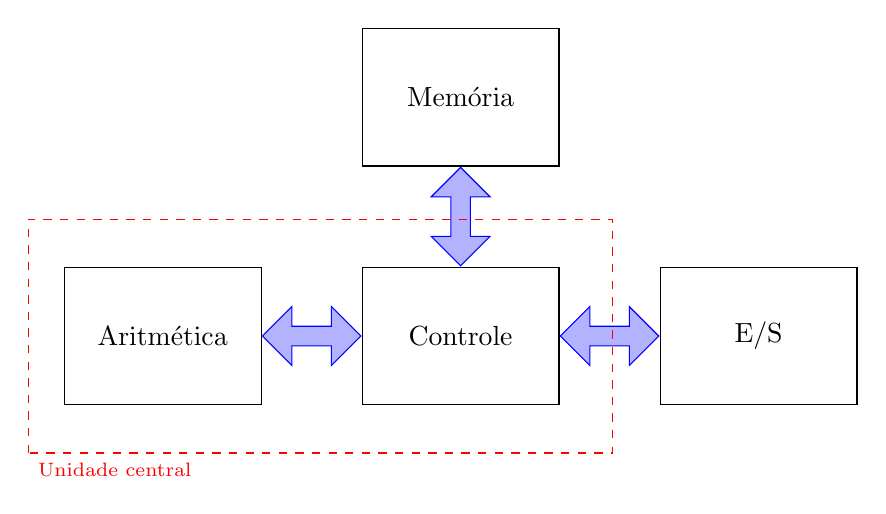
\begin{tikzpicture}[scale=0.9,
  module/.style={anchor=west,draw,rectangle,minimum width=\width,minimum height=\height},
  vdarrow/.style={anchor=west,double arrow,draw=blue,fill=blue!30,minimum height=1.25cm}, % vertical double arrow
  hdarrow/.style={vdarrow,rotate=90} % horizontal double arrow
  ]
  \node[name=a,module] at (0,0) {Aritm\'etica};
  \node[name=ac,vdarrow,shift=(a.east)] {};
  \node[name=c,module,shift=(ac.east)] {Controle};
  \node[name=ces,vdarrow,shift=(c.east)] {};
  \node[name=es,module,shift=(ces.east)] (es) at (2*\height+2*\width,0) {E/S};
  % ATENTION HERE: rotating the double arrow dont change
  % the position names, so east continues being the extremity
  \node[name=ces,hdarrow,shift=(c.north)] {};
  \node[name=mem,module,anchor=south,shift=(ces.east)] {Mem\'oria};
  \draw[dashed,draw=red] (-0.5,-1.65) node[below right]
  {\color{red}{\scriptsize{Unidade central}}} rectangle (7.75,1.65);
\end{tikzpicture}

\end{frame}

\subsection{Mark 1}

\begin{frame}{Manchester Mark 1}
  \begin{columns}
    \begin{column}{.45\textwidth}
      \includegraphics[scale=.5]{\imgdir/manchester-mark1.png}
    \end{column}

    \begin{column}{.55\textwidth}
      \begin{itemize}
      \item Projetistas:
        \href{http://en.wikipedia.org/wiki/Frederic_Calland_Williams}{Frederic
          C. Williams} e \href{Tom Kilburn}{Tom Kilburn};
      \item Desenvolvido na Universidade de Vitória em Manchester
        tornando-se operacional em {\bf 1949};
      \item Continha inovações como programas armazenados em
        memória e registradores para armazenar índices das instruções;
      \item Possuía palavra de 40 bits com byte de 5 bits.
      \end{itemize}
    \end{column}
  \end{columns}

  \begin{itemize}
  \item Contou com a consultoria de Alan Turing que posteriormente
    produziria o
    \href{http://www.digital60.org/documents/turing.png}{manual para o
      Mark II}.
  \end{itemize}
\end{frame}

